\documentclass[11pt,a4paper]{article}

% --- Packages ---
\usepackage[utf8]{inputenc}
\usepackage[margin=1in]{geometry}
\usepackage[breaklinks=true,colorlinks,citecolor=blue,linkcolor=blue,urlcolor=blue]{hyperref}
\usepackage[table,xcdraw]{xcolor}
\usepackage{epsfig, mathrsfs, latexsym, subfigure, marginnote, gensymb, amsmath}
\usepackage{graphicx}
\usepackage{booktabs}
\usepackage{adjustbox}
\usepackage{doi}

% Package to handle multiple authors and affiliations cleanly in the article class
\usepackage{authblk}

% --- Metadata ---
\title{\textbf{Supporting Information for ``pydemi: Interpretable Charge-Density Descriptors from DFT or Machine-Learned Densities, and What They Add to Materials Property Prediction''}}

\author[1]{Shubham Kumar Maurya}
\author[1]{Somnath Bhowmick\thanks{bsomnath@iitk.ac.in}}
\affil[1]{Department of Materials Science \& Engineering, Indian Institute of Technology Kanpur, Kanpur 208016, India}

\date{\today}

% --- Document Start ---
\begin{document}

\renewcommand{\thesection}{S\arabic{section}}
\renewcommand{\thetable}{S\arabic{table}}
\renewcommand{\thefigure}{S\arabic{figure}}
\renewcommand{\theequation}{S\arabic{equation}}
\newcommand{\dn}[1]{\texttt{\detokenize{#1}}}

\maketitle

All numbers and tables in this document are generated by the scripts in
\texttt{paper/analysis/} of the repository from the files they name.

% ==========================================================================
\section{Descriptor definitions}
\label{si:defs}

\paragraph{Notation.} The cell of volume $V$ is divided into $N_v$ voxels $k$ of
volume $\Delta V=V/N_v$; $\rho_k$ is the density in e\,\AA$^{-3}$ (the
\texttt{CHGCAR} value divided by $V$), $Q_\mathrm{tot}=\sum_k\rho_k\Delta V$ and
$\langle\rho\rangle=Q_\mathrm{tot}/V$. For each voxel, $i(k)$ is the nearest
nucleus (periodic images included), $r_k$ its distance and $\hat{\mathbf u}_k$
the unit vector from that nucleus to the voxel. The core, bond and interstitial
shells are $r_k\le c_1$, $c_1<r_k\le c_2$ and $r_k>c_2$ (defaults $c_1=0.8$\,\AA,
$c_2=1.5$\,\AA). $\nabla\rho$, $\nabla^2\rho$ and the Hessian eigenvalues
$\lambda_1\le\lambda_2\le\lambda_3$ are computed spectrally on the periodic grid.
Quantities defined in atomic units (NCI, information measures) are evaluated in
bohr. A descriptor that is undefined for a special input returns a documented
constant and sets a flag.

\subsection{Bonding (19)}
\begin{description}
\item[\dn{m1}, \dn{m2}, \dn{sigma_r2}] [\AA, \AA$^2$, \AA$^2$]
$m_n=\sum_k\rho_k r_k^n/\sum_k\rho_k$, $\sigma_r^2=m_2-m_1^2$: mean distance of
the charge from its nearest nucleus, second moment and radial spread.
\item[\dn{f_core}, \dn{f_bond}, \dn{f_int}] fraction of the charge in the core,
bond and interstitial shells; they sum to one.
\item[\dn{zeta}] [0--1] $\zeta=1-\sum_k|\nabla\rho_k\cdot\hat{\mathbf u}_k|/\sum_k|\nabla\rho_k|$:
zero for spherical, non-overlapping atoms.
\item[\dn{lnf}] $N_v^{-1}\sum_k\mathbf 1[\nabla^2\rho_k<0]$: volume fraction where
charge is concentrated.
\item[\dn{lnf_charge_weighted}] $\sum_{\nabla^2\rho_k<0}\rho_k/\sum_k\rho_k$: the
same as a charge fraction.
\item[\dn{lap_concentration}] $\sum_{\nabla^2\rho_k<0}|\nabla^2\rho_k|/\sum_k|\nabla^2\rho_k|$;
identically $\tfrac12$ on a periodic grid, kept for completeness.
\item[\dn{lap_concentration_valence}] the same ratio over the voxels with
$r_k>c_1$.
\item[\dn{ellip_bond_bounded_avg}] [0--1) mean of $1-\lambda_2/\lambda_1=\varepsilon/(1+\varepsilon)$
over the bond-shell voxels with $\lambda_2<0$: zero for cylindrical charge.
\item[\dn{f_NCI}] volume fraction of the NCI region
$\{s_k<0.5,\ \rho_k<0.05$ a.u.$\}$, with
$s=|\nabla\rho|/\big(2(3\pi^2)^{1/3}\rho^{4/3}\big)$.
\item[\dn{NCI_attractive}] fraction of the NCI voxels with $\lambda_2<0$.
\item[\dn{sign_lambda2_rho_mean}] [e\,bohr$^{-3}$] mean of
$\mathrm{sign}(\lambda_2)\rho$ over the NCI region.
\item[\dn{V_spread}, \dn{V_int_min}] [eV] standard deviation of the Hartree
potential energy $V(\mathbf G)=4\pi k_e\rho(\mathbf G)/|\mathbf G|^2$ (cell
average zero) over the atomic sites; its minimum in the interstitial shell.
\item[\dn{rho_mid_mean}, \dn{rho_mid_std}] [e\,\AA$^{-3}$] mean and standard
deviation of $\rho$, by Fourier interpolation, at the midpoints of the
first-shell bonds ($|\mathbf R_{ij}|\le1.1\,d_i$, $d_i$ the nearest-neighbour
distance of atom $i$).
\end{description}

\subsection{Structural (19)}
\begin{description}
\item[\dn{rho_perc_a}, \dn{rho_perc_b}, \dn{rho_perc_c}] [e\,\AA$^{-3}$]
$\max\{c:\{\rho>c\}$ contains a cluster that winds around the cell along
$\mathbf a_\alpha\}$: density at the bottleneck of the best connecting path.
\item[\dn{perc_anisotropy}] $(\max_\alpha-\min_\alpha)\rho_{\mathrm{perc},\alpha}/\mathrm{mean}_\alpha\rho_{\mathrm{perc},\alpha}$.
\item[\dn{n_max}, \dn{n_min}] [\AA$^{-3}$] voxels higher (lower) than all 26
neighbours, per volume.
\item[\dn{n_NNM}, \dn{Q_NNM}] maxima farther than 0.8\,\AA{} from every nucleus,
per volume [\AA$^{-3}$]; charge in their steepest-ascent basins over
$Q_\mathrm{tot}$.
\item[\dn{rho_min}, \dn{rho_min_ratio}, \dn{rho_int_mean}] $\min_k\rho_k$
[e\,\AA$^{-3}$]; $\rho_{\min}/\langle\rho\rangle$; mean $\rho$ over the
interstitial shell [e\,\AA$^{-3}$].
\item[\dn{T_eigenvalues_t1}, \dn{_t2}, \dn{_t3}] sorted eigenvalues of
$T_{ab}=\sum_k\partial_a\rho_k\partial_b\rho_k/\sum_k|\nabla\rho_k|^2$ (trace 1;
all $\tfrac13$ for a cubic crystal).
\item[\dn{charge_FA}] [0--1] $\sqrt{3/2}\,\lVert T-\tfrac13I\rVert_F/\lVert T\rVert_F$.
\item[\dn{shannon_entropy}] $S=-\int\tilde\rho\ln\tilde\rho\,dV-\ln V$ with
$\tilde\rho=\rho/N_e$; zero for a uniform density.
\item[\dn{disequilibrium}] $D=V\int\tilde\rho^{\,2}\,dV$; one for a uniform density.
\item[\dn{LMC_complexity}] $C=De^{S}$.
\item[\dn{fisher_information}] [bohr$^{-2}$] $I=\int|\nabla\tilde\rho|^2/\tilde\rho\,dV$.
\end{description}

\subsection{Site heterogeneity (18)}
Each voxel is assigned to an atom with weight $w_i(k)$ (nearest atom by default;
power diagram or Becke cells optionally), and three per-atom quantities are
computed:
\begin{equation}
m_1^{(i)}=\frac{\sum_k w_i(k)\rho_k r_{ik}}{\sum_k w_i(k)\rho_k},\quad
f_\mathrm{bond}^{(i)}=\frac{\sum_{c_1<r_{ik}\le c_2}w_i(k)\rho_k}{\sum_k w_i(k)\rho_k},\quad
\zeta^{(i)}=1-\frac{\sum_k w_i(k)|\nabla\rho_k\cdot\hat{\mathbf u}_{ik}|}{\sum_k w_i(k)|\nabla\rho_k|}.
\end{equation}
For each $X\in\{m_1,f_\mathrm{bond},\zeta\}$ the descriptors are
\dn{X_site_std} ($\mathrm{std}_iX^{(i)}$), \dn{X_site_range}, \dn{X_site_max},
\dn{X_site_min}, \dn{X_within_element_var}
($\sum_e x_e\mathrm{Var}_{i\in e}X^{(i)}$) and \dn{X_between_element_var}
($\sum_e x_e(\bar X_e-\bar X)^2$), with $x_e$ the site fraction of element $e$;
the last two add up to $\mathrm{Var}_iX^{(i)}$. The within-element variance is NaN
(flagged) when no element has two or more sites, and the between-element
variance is zero (flagged) for an elemental crystal.

% ==========================================================================
\section{Sensitivity and transfer per descriptor}
\label{si:stability}

\begin{table}[htbp]
\centering
\caption{Median relative change (\%) of each descriptor when the grid is
coarsened to 80\% per axis, the FFT derivatives are replaced by fourth- or
second-order differences, and the nearest-atom partition by the power diagram
or Becke cells (sample sizes as in Fig.~3 of the main text; -- = does not depend
on the choice), and the Spearman correlation $\rho_s$ and median relative error
(\%) between the descriptors of the DFT and ChargE3Net-predicted densities of the
605 test structures. Relative change: $|a-b|/\max(|a|,|b|)$.}
\label{tab:si_stability}
\footnotesize
\begin{tabular}{lccccccc}
\toprule
Descriptor & grid 80\% & FD4 & FD2 & power & Becke & $\rho_s$ (ML) & ML error \\
\midrule
\csname @@input\endcsname tables/tab_si_descriptors.tex 
\bottomrule
\end{tabular}
\end{table}

% ==========================================================================
\section{Property models}
\label{si:props}

\paragraph{Targets.} The bulk, shear and Young's moduli (Voigt--Reuss--Hill),
the Poisson ratio, the energy relative to the free atoms ($E_\mathrm{form}$ of
the benchmark) and its Debye temperature are taken from the property table of the
cross-model benchmark of S.~K.~Maurya and S.~Bhowmick (manuscript in preparation); Poisson ratios $\geq0.5$
were removed. All other targets come from the Materials Project, database
version 2026.04.13, for the same material identifiers. Elastic data were kept
only where $K$ and $G$ lie between 0 and 1000\,GPa and agree with the benchmark
table (6,000 materials); $C_{11}$, $C_{12}$, $C_{44}$ and the anisotropy index
$A^U=5G_V/G_R+K_V/K_R-6$ only where the smallest eigenvalue of the unrounded
stiffness tensor exceeds 1\,GPa (5,791), with $A^U$ computed from that tensor.
The direct-gap label is defined only for materials with a gap (1,836).

\paragraph{Training.} Composition: matminer \texttt{Stoichiometry} ($p$-norms
for $p=0,2,3,5,7,10$) and \texttt{ElementProperty} with the Magpie preset
(22 elemental properties $\times$ minimum, maximum, range, mean, average
deviation, mode), 138 features. Descriptors: the 56 of pydemi without the
constant Laplacian concentration ratio. Ridge and logistic regression: median
imputation, standardization, penalty from $10^{-3}$ to $10^{3}$ (13 values)
chosen on the validation set. Random forests: 500 trees, $\frac13$ of the
features per split for regression and $\sqrt{n}$ for classification, median
imputation. LightGBM: missing values handled natively; 50 Optuna TPE trials
(sampler seed 0) over learning rate 0.01--0.1 (log), 7--127 leaves (log),
minimum leaf size 5--100 (log), feature fraction 0.3--1, bagging fraction
0.5--1 and $L_1$, $L_2$ penalties $10^{-8}$--10 (log); objective the squared
error of the (transformed) target or the log-loss; early stopping after 200
rounds without improvement on the validation set, at most 10,000 rounds.
$\log_{10}$ was applied to $\varepsilon$, $\varepsilon_\infty$ and $n$,
$\log(1+x)$ to $\varepsilon_\mathrm{ion}$ and $A^U$. Nine of the 75 LightGBM
configurations used more than 9,500 rounds on average, so a larger cap could
improve them slightly. SHAP values are the exact tree contributions of LightGBM
on the test set, averaged over the seeds.

\begin{table}[htbp]
\centering
\caption{LightGBM with descriptors and composition: test MAE (mean $\pm$
standard deviation over five seeds), RMSE, $R^2$ (ROC-AUC for the
classifications) of the five-seed ensemble, accuracy, and mean number of
boosting rounds.}
\label{tab:si_lgbm}
\begin{adjustbox}{width=\textwidth}
\begin{tabular}{llccccr}
\toprule
Property & Units & MAE & RMSE & Ensemble $R^2$ / AUC & Accuracy & Rounds \\
\midrule
\csname @@input\endcsname tables/tab_si_lgbm.tex 
\bottomrule
\end{tabular}
\end{adjustbox}
\end{table}

\begin{table}[htbp]
\centering
\caption{Test $R^2$ (ROC-AUC for the classifications) of every model and
feature set, mean over five seeds (ridge: one fit). C: composition (138), D:
pydemi descriptors (55), D+C: both (193).}
\label{tab:si_full}
\begin{adjustbox}{width=\textwidth}
\begin{tabular}{lccccccccc}
\toprule
 & \multicolumn{3}{c}{Ridge / logistic} & \multicolumn{3}{c}{Random forest} & \multicolumn{3}{c}{LightGBM} \\
\cmidrule(lr){2-4} \cmidrule(lr){5-7} \cmidrule(lr){8-10}
Property & C & D & D+C & C & D & D+C & C & D & D+C \\
\midrule
\csname @@input\endcsname tables/tab_si_full.tex 
\bottomrule
\end{tabular}
\end{adjustbox}
\end{table}

\begin{table}[htbp]
\centering
\caption{Models distributed for \texttt{pydemi.props}: mean validation loss of
LightGBM over the seeds for each feature set (RMSE of the transformed target, or
log-loss), the feature set chosen, and the hyperparameters and number of rounds
of the seed-0 model.}
\label{tab:si_selection}
\begin{adjustbox}{width=\textwidth}
\begin{tabular}{lccccccccr}
\toprule
Property & val.\ C & val.\ D & val.\ D+C & chosen & learning rate & leaves & min.\ leaf & feature fraction & rounds \\
\midrule
\csname @@input\endcsname tables/tab_si_selection.tex 
\bottomrule
\end{tabular}
\end{adjustbox}
\end{table}

% ==========================================================================
\section{Properties from predicted densities}
\label{si:mlprops}

For the 605 test structures of the density model, the distributed property models
were evaluated with the descriptors of the DFT and of the predicted densities
(composition unchanged). Agreement: $R^2$ between the two predictions and their
median relative difference over all 605 (for the classifications, the share of
structures with the same class). Accuracy: against the target values for the 63
structures (fewer where the target is missing) that are also in the test set of
the property models.

\begin{table}[htbp]
\centering
\caption{Property predictions from DFT and predicted descriptors. Inputs: C
composition, D descriptors, D+C both; for the C models the two predictions are
identical by construction.}
\label{tab:si_mlprops}
\begin{adjustbox}{width=\textwidth}
\begin{tabular}{llccccccc}
\toprule
 & & \multicolumn{2}{c}{Agreement (605)} & & \multicolumn{2}{c}{$R^2$ / AUC} & \multicolumn{2}{c}{MAE} \\
\cmidrule(lr){3-4} \cmidrule(lr){6-7} \cmidrule(lr){8-9}
Property & Inputs & $R^2$ & diff.\ (\%) / same class (\%) & $n$ & DFT desc. & ML desc. & DFT desc. & ML desc. \\
\midrule
\csname @@input\endcsname tables/tab_si_mlprops.tex 
\bottomrule
\end{tabular}
\end{adjustbox}
\end{table}

% ==========================================================================
\section{Graphical interface}
\label{si:gui}

\begin{figure}[htbp]
\centering
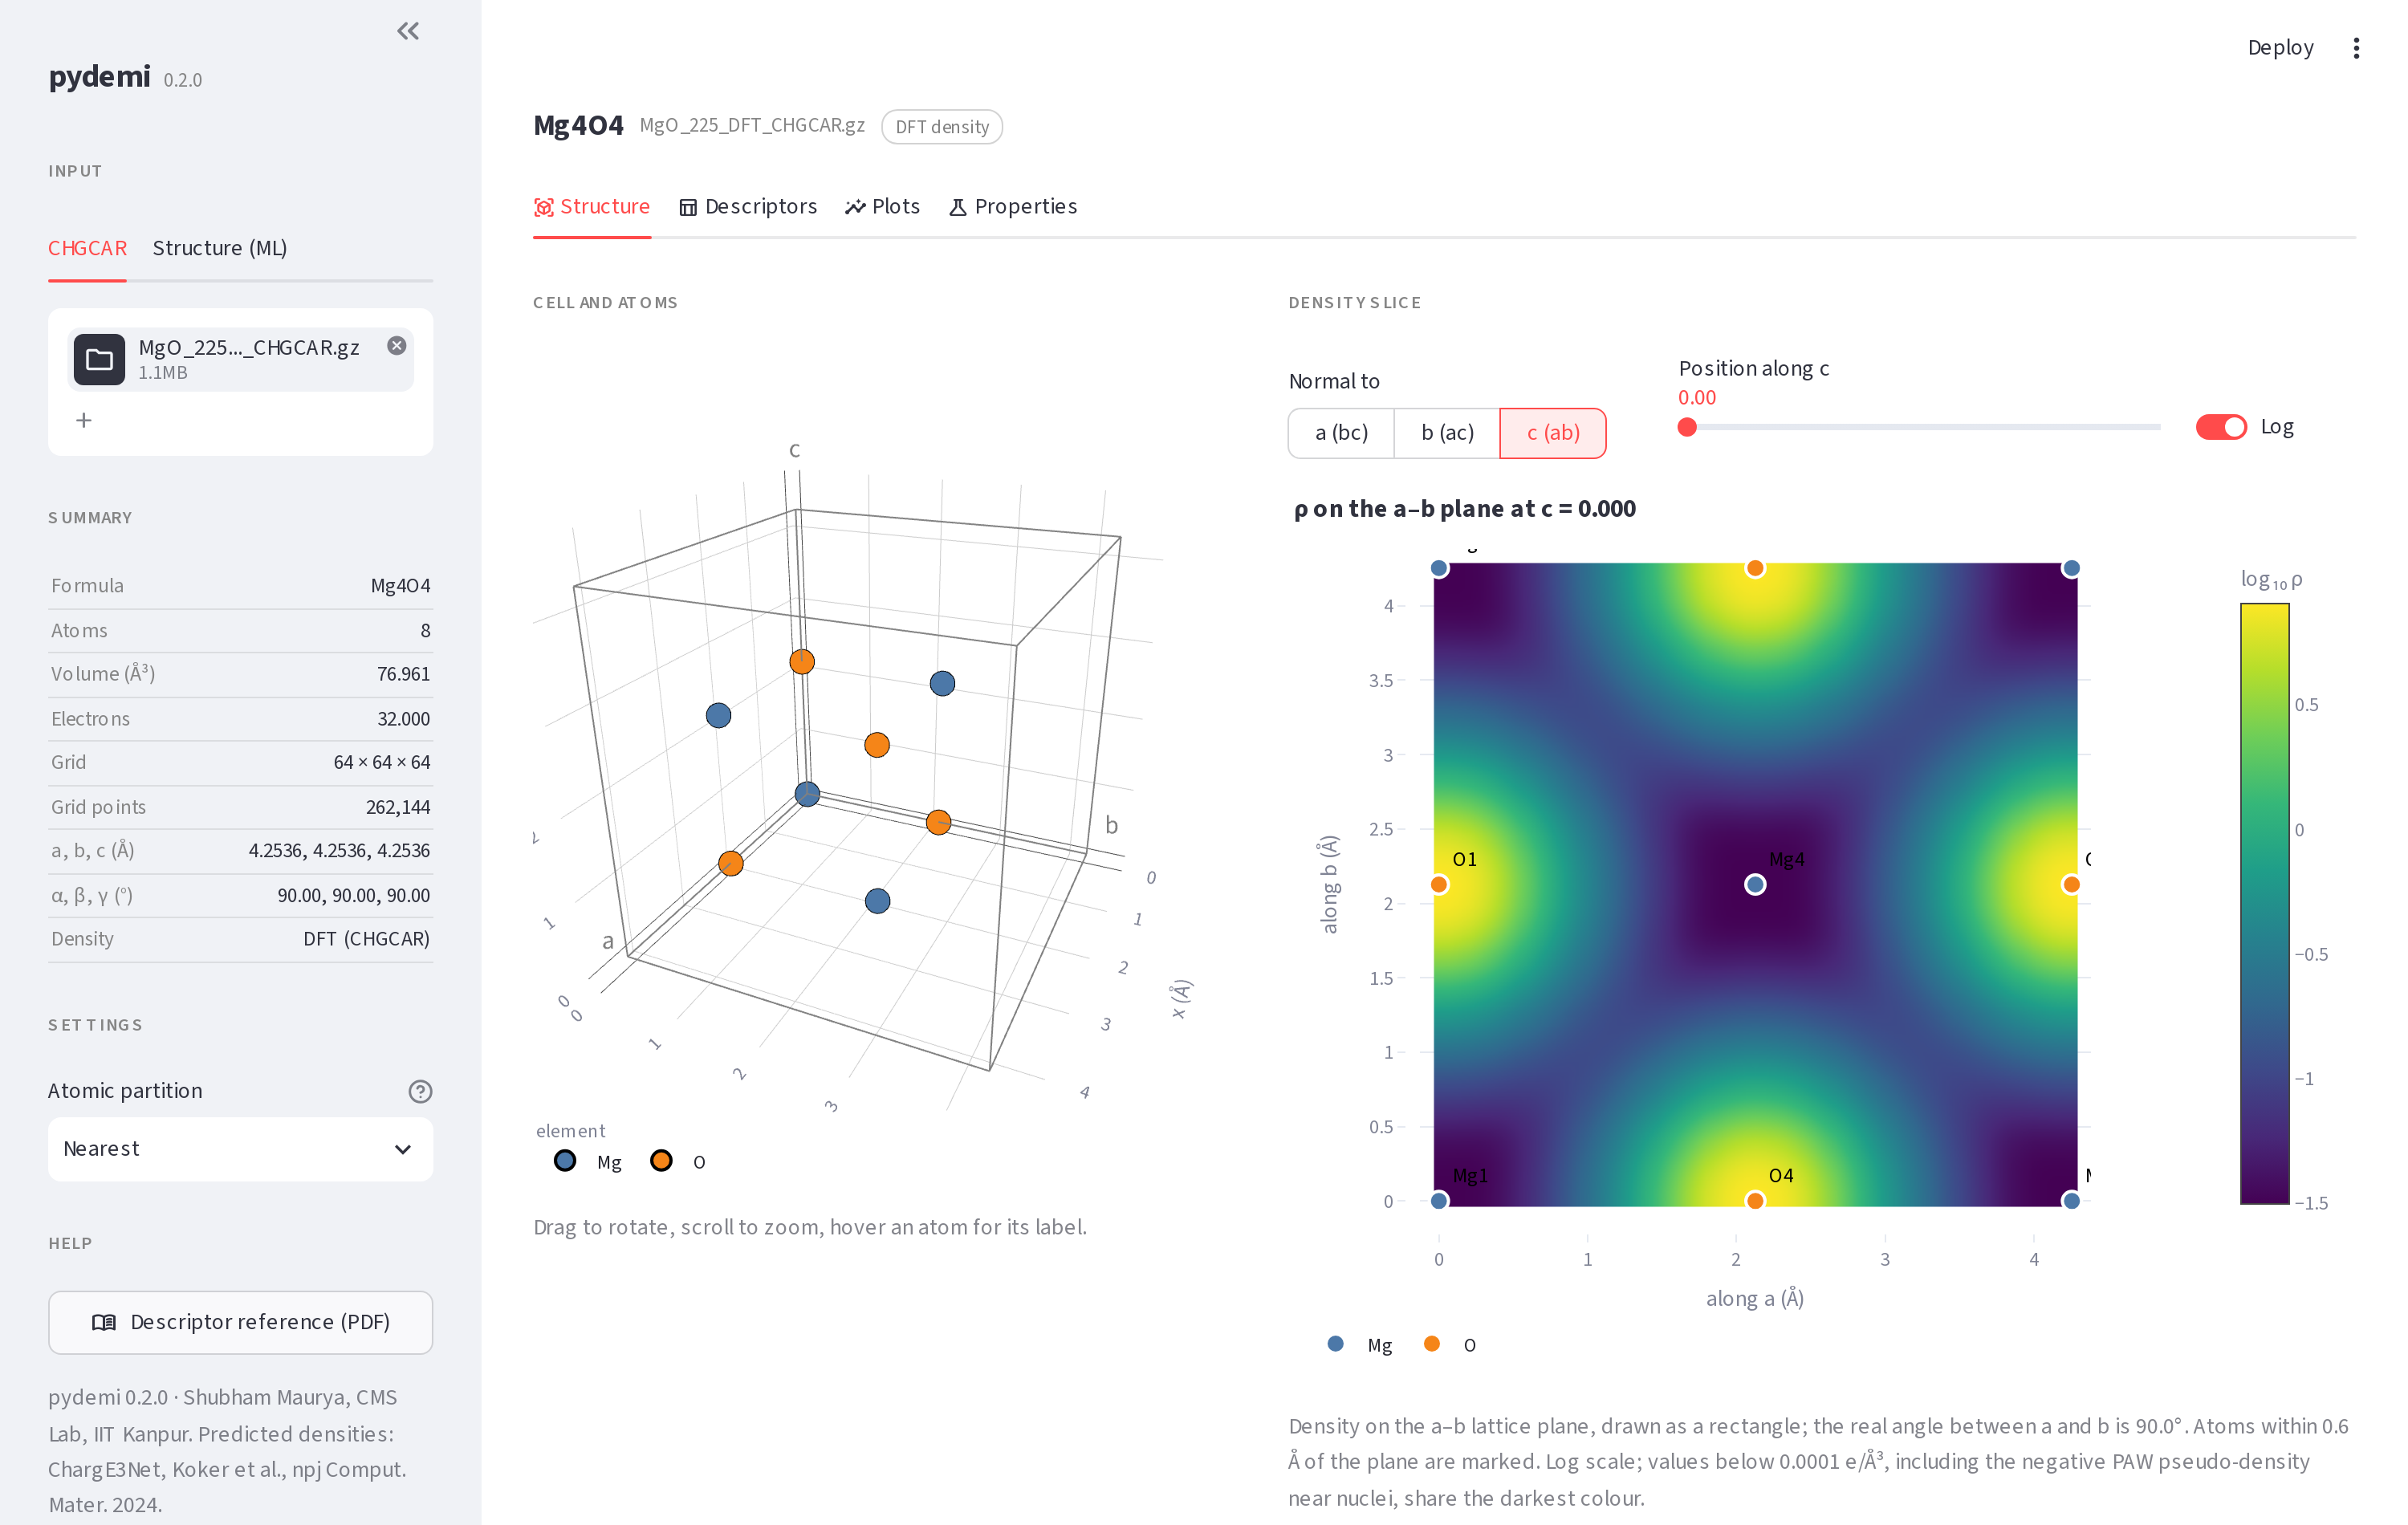
\includegraphics[width=\textwidth]{figures/fig_gui_structure.png}
\caption{Structure view of the graphical interface for MgO: the cell and atoms
in 3D and a slice of the density through a lattice plane (logarithmic colour
scale; atoms within 0.6\,\AA{} of the plane marked). The input panel on the
left offers a \texttt{CHGCAR} or, in the \emph{Structure (ML)} tab, a structure
file whose density is predicted.}
\label{fig:si_gui}
\end{figure}

\end{document}
